\documentclass[a4paper, 12pt]{article}%тип документа

%отступы
\usepackage[left=1.5cm,right=1cm,top=2cm,bottom=3cm,bindingoffset=0cm]{geometry}
\setlength{\parindent}{5ex}
%Русский язык
\usepackage[T2A]{fontenc} %кодировка
\usepackage[utf8]{inputenc} %кодировка исходного кода
\usepackage[english,russian]{babel} %локализация и переносы

%Вставка картинок
\usepackage{graphicx}
\graphicspath{{pictures/}}
\DeclareGraphicsExtensions{.pdf,.png,.jpg,}
\usepackage{wrapfig}

%Графики
\usepackage{pgfplots}
\pgfplotsset{compat=1.9}

%Математика
\usepackage{amsmath, amsfonts, amssymb, amsthm, mathtools}

%Таблицы
\usepackage{longtable} 
\usepackage{float}

%Римские цифры
\newcommand{\RomanNumeralCaps}[1]{\uppercase\expandafter{\romannumeral#1}}

\usepackage{multirow}



\begin{document}
	\begin{titlepage}
		\begin{center}
			\textsc{Федеральное государственное автономное образовательное учреждение высшего образования«Московский физико-технический институт (национальный исследовательский университет)»\\[5mm]
			}
			
			\vfill
			
			\textbf{Отчёт по лабораторной работы 4.3.2\\[3mm]
				Дифракция света на ультразвуковой волне
				в жидкости
				\\[50mm]
			}
			
		\end{center}
		
		\hfill
		\begin{minipage}{.5\textwidth}
			Выполнил студент:\\[2mm]
			Сериков Василий Романович\\[2mm]
			группа: Б03-102\\[5mm]
			
		\end{minipage}
		\vfill
		\begin{center}
			Москва, 2023 г.
		\end{center}
		
	\end{titlepage}
	
	\newpage
	\setcounter{page}{2}
	\textbf{Аннотация}\\
	
	\textbf{Цель работы: }\\
	
	Изучение дифракции света на синусоидальной акустической решётке и наблюдение фазовой решётки методом тёмного
	поля.\\
	
	\textbf{Приборы: }\\
	
	Оптическая скамья, осветитель, два длиннофокусных объектива, кювета с жидкостью, кварцевый излучатель
	с микрометрическим винтом, генератор ультразвуковой частоты, линза, вертикальная нить на рейтере, микроскоп.\\
	
	\textbf{Теория: }\\
	
	При прохождении ультразвуковой волны через жидкость в ней возникают периодические неоднородности коэффициента преломления, создается фазовая решетка, которую мы считаем неподвижной ввиду малости скорости звука относительно скорости света. Показатель
	преломления n изменяется по закону:
	
	\begin{equation}\label{}
		n = n_0 (1 + m \cos \Omega x)
	\end{equation}
	
	Здесь $ \Omega = 2 \pi / \Lambda $ --- волновое число для ультразвуковой волны, $ m $ --- глубина модуляции $ n $ $ (m \ll 1 $).
	
	Положим фазу $ \phi $ колебаний световой волны на передней стенке кюветы равной нулю, тогда на задней поверхности она равна:
	
	\begin{equation}\label{}
		\phi  = k n L = \phi_0 (1 + m \cos \Omega x)
	\end{equation}
	
	Здесь $ L $ --- толщина жидкости в кювете, $ k = 2 \pi / \lambda $ --- волновое число для света.
	
	После прохождения через кювету световое поле есть совокупность плоских волн, распространяющихся под углами $ \theta $, соответствующими максимумам в дифракции Фраунгофера:
	
	\begin{equation}\label{}	
		\Lambda \sin \theta_m = m \lambda
	\end{equation}
	
	Этот эффект проиллюстрирован на рисунке 1.
	\begin{figure}[h!]
		\centering	
		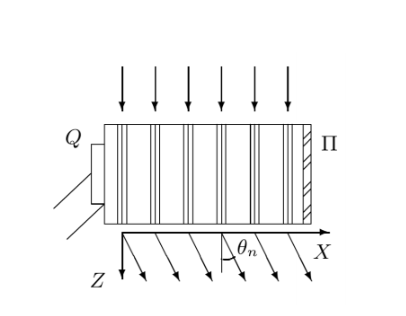
\includegraphics[width=0.3\textwidth]{wave.png}
		\caption{Дифракция световых волн на акустической решетке}
		\label{diff}
	\end{figure}
	Зная положение дифракционных максимумов, по формуле (1) легко определить длину ультразвуковой волны, учитывая малость $ \theta $: $ \sin \theta \approx \theta \approx l_m /F  $, где $ l_m $ --- расстояние от нулевого до последнего видимого максимума, $ F $ --- фокусное расстояние линзы. Тогда получим:
	
	\begin{equation}\label{}
		\Lambda = m \lambda F/ l_m 
	\end{equation}
	Скорость ультразвуковых волн в жидкости, где $ \nu $ --- частота колебаний излучателя:
	
	\begin{equation}\label{}
		v = \Lambda \nu 
	\end{equation}
	Схема установки приведена на рисунке 2. Источник света Л через светофильтр Ф и конденсор К освещает вертикальную щель $ S $, находящуюся в фокусе объектива $ O_1 $. После объектива параллельный световой пучок проходит через кювету С перпендикулярно акустической решетке, и дифракционная картина собирается в фокальной плоскости объектива $ O_2 $ , наблюдается при помощи микроскопа М.
	Фокусное расстояние объектива $F = 28 $ см, одно деление винта микроскопа составляет 50~мкм, полоса пропускания фильтра \mbox{$\lambda = 6400\pm 200$ Å}, цена деления лимба 10 мкм.
	
	\begin{figure}[h!]
		\centering	
		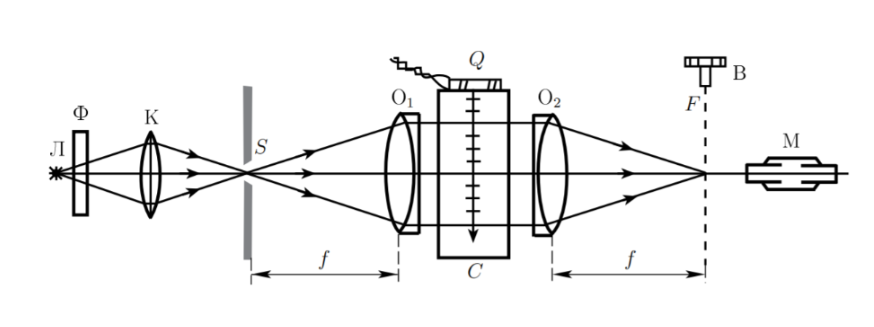
\includegraphics[width=0.7\textwidth]{stand.png}
		\caption{Схема установки}
		\label{shema1}
	\end{figure}

	\begin{figure}[h!]
	\centering	
	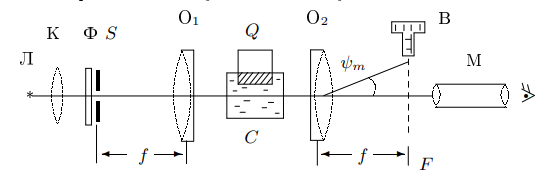
\includegraphics[width=0.7\textwidth]{acustic.png}
	\caption{Схема для наблюдения дифракции на акустической решетке}
	\end{figure}

	\newpage
	\textbf{Ход работы: }\\
	
	\begin{enumerate}
		\item Перемещая излучатель с помощью лимба, оценим по порядку величины длину $\lambda$ УЗ-волны как удвоенное расстояние между наиболее чёткими дифракционными картинами, определим положения дифракционных полос и рассчитаем длину УЗ-волны $\Lambda$ по формуле 3. Полученные значения занесем в таблицы 1 и 2.
		
		\begin{longtable}{|c|c|c|c|c|c|c|}
			\hline
			№              & 1    & 2    & 3    & 4    & 5    & 6    \\ \hline
			$\lambda$, мкм & 1560 & 1520 & 1000 & 1000 & 840  & 760  \\ \hline
			$\Lambda$, мкм & 1600 & 1400 & 1050 & 896  & 792  & 712  \\ \hline
			$\nu$, кГц     & 900  & 1100 & 1400 & 1600 & 1800 & 2000 \\ \hline
			$m$            & 2    & 3    & 2    & 1    & 1    & 1    \\ \hline
			\caption{Полученные данные из эксперимента с дифракцией на УЗ-волне. $\sigma_{\lambda} = 10$ мкм, $\varepsilon_{\Lambda}$ = 5\%, $\sigma_{\nu} = 10$ кГц}
		\end{longtable}
	
		\begin{longtable}{|c|c|c|c|c|c|c|}
			\hline
			m \ №  & 1   & 2   & 3 & 4 & 5  & 6    \\ \hline
			3, мкм & -   & 384 & - & - & -  & -    \\ \hline
			2, мкм & 228 & 250 & 342 & - & -  & -  \\ \hline
			1, мкм & 111 & 128 & 171 & 200 & 226 & 250 \\ \hline
			\caption{Полученные значения расстояния l от нулевого максимума до m-того. $\sigma_l = 10$ мкм}
		\end{longtable}
	
	
	\item Рассчитаем скорости звука в воде по полученным значениям по формуле $v = \Lambda \nu$. 
	
	\begin{longtable}{|c|c|c|c|c|c|c|c|}
		\hline
		m \ №  & 1 & 2 & 3 & 4 & 5 & 6  &  $\overline{v}$ \\ \hline
		$v$, м/с & 1440 & 1540 & 1470 & 1433 & 1425 & 1424 & 1455 \\ \hline
		\caption{Полученные значения скорости звука в воде. $\varepsilon_v = 5\% $}
	\end{longtable}
	
		\begin{figure}[H]
		\centering	
		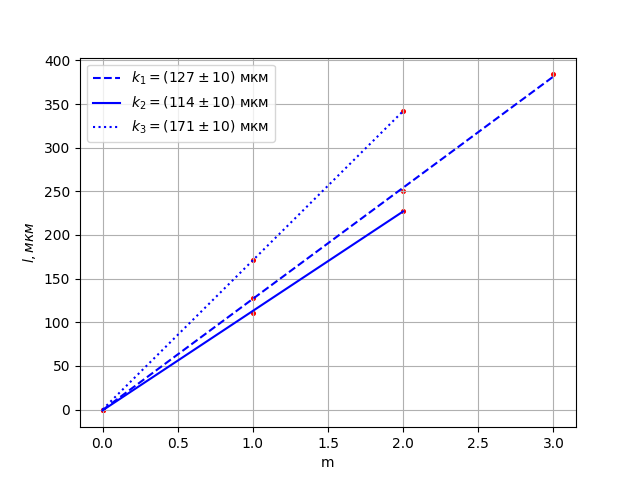
\includegraphics[width=0.8\textwidth]{l(m).png}
		\caption{График зависимости l(m) по полученным значения расстояния от полосы до нуля}
	\end{figure}
	
	
	\item Определим скорость распространения УЗ-волны в воде методом темного поля. Для этого закроем проволокой центральный максимум и определим период полученной решетки при фиксированных частотах. Зафиксируем с помощью окулярной шкалы микроскопа разность координат N первой и последней из хорошо видимых в поле зрения тёмных полос
	и количество m светлых промежутков между ними. По полученным данным рассчитаем длину волны $\Lambda$, построим график зависимости $\Lambda = f(1/\nu)$ и по коэффициенту наклона прямой определим скорость звука в воде.
	
	$$ \Lambda/2 = \frac{N}{m - 1} $$
	\begin{longtable}{|c|c|c|c|}
		\hline
		$\nu$, МГц  & N, мм  & m  & $\Lambda$, мкм    \\ \hline
		1 & 3,1 & 10 & 688 $\pm 68$    \\ \hline
		1,2 & 4,4 & 16 & 586 $\pm 39$  \\ \hline
		1,4 & 4,1 & 17 & 512 $\pm 30$  \\ \hline
		1,6 & 4,0 & 19 & 444 $\pm 25$  \\ \hline
		1,8 & 4,4 & 23 & 400 $\pm 20$  \\ \hline
		2   & 3,6 & 22 & 342 $\pm 16$  \\ \hline
		\caption{Полученные значения для разности координат, числа максимумов и периода решетки. $\sigma_m = 1$, $\sigma_N = 0,1$ мм}
	\end{longtable}
	
	\begin{figure}[h!]
		\centering	
		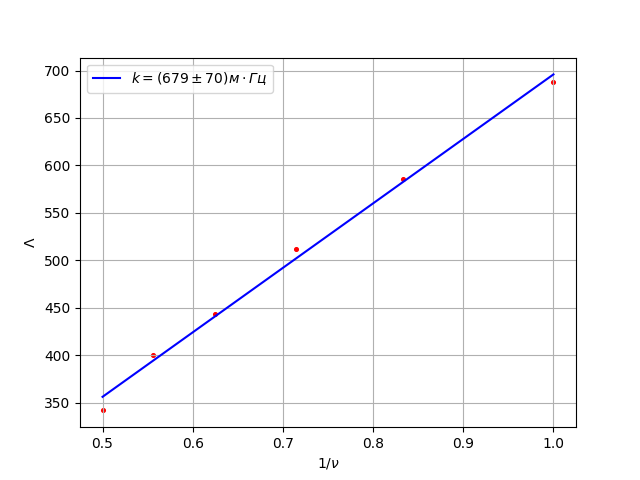
\includegraphics[width=0.8\textwidth]{L(nu).png}
		\caption{График зависимости $\Lambda(1/\nu)$, k = v - скорость звука в воде.}
	\end{figure}
	
	
	\end{enumerate}
	
	
	
	\textbf{Обсуждение результатов и выводы: }\\
	
	В ходе данной работы мы изучили явление дифракции света на синусоидальной акустической решетке и наблюдали фазовую решетку методом темного поля.
	
	Расчет значения скорости звука в воде с помощью акустической решетки v = 1445$\pm 70$ м/с сходится с теоретическим v = 1490 м/с.
	
	Расчет значения скорости звука методом темного поля v = 679$\pm 70$ м/с не сходится с теоретическим значением, это может быть связано с неправильным снятием данных расстояния между максимумами дифракционной картины.
	
	
	
	
	
	
	
	
	
	
	
	
	
	
	
	
	
	
	
	
	
	
	
	
	
	
	
	
	
	
	
	
	
	
	
	
	
	
	
	
	
	
	
	
	
	
	
	\end{document}